\documentclass[18pt]{article}
\usepackage[utf8]{inputenc}
\usepackage[T1]{fontenc}
\usepackage{ragged2e}
\usepackage{caladea}
\usepackage{graphicx}
\usepackage{longtable}
\usepackage{wrapfig}
\usepackage{rotating}
\usepackage{epigraph}
\usepackage[normalem]{ulem}
\usepackage{hyperref}
\usepackage{amsmath}
\usepackage{amssymb}
\usepackage{capt-of}
\usepackage{hyperref}
\usepackage{fancyhdr}

\title{
 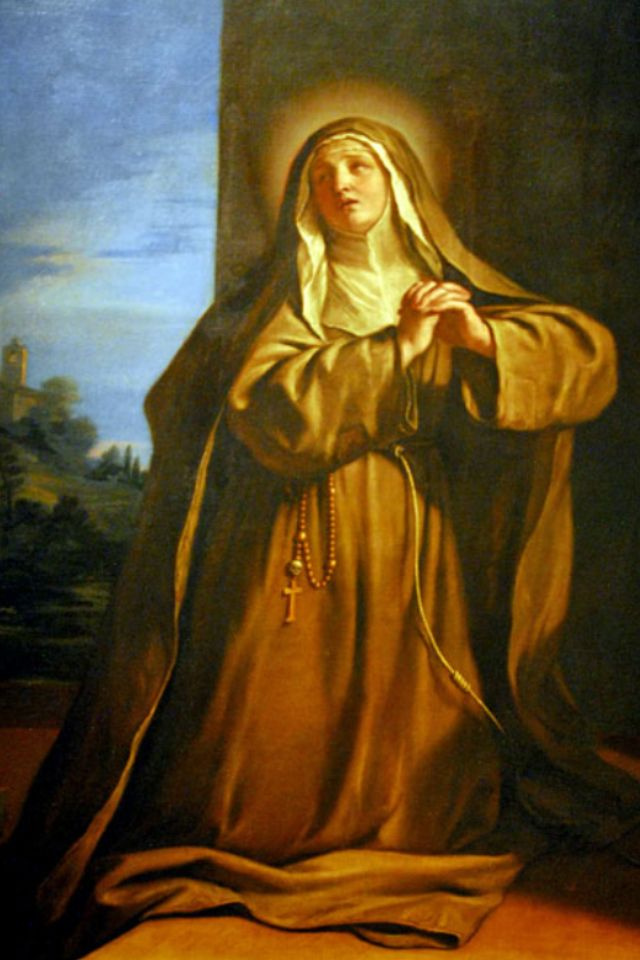
\includegraphics[scale=0.45, trim={10cm, 0, 10cm, 0}]{./assets/imagem.jpg}
  \par
   NOVENA A SANTA MARGARIDA DE CORTONA}
\date{Início da Novena: 13/02 - Data Litúrgica: 21/02 }

% Comando para fazer "Sumário" não aparecer no Sumário.
\renewcommand{\contentsname}{Sumário}
\begin{document}
\maketitle

\thispagestyle{empty} %zera a primeira página

\pagestyle{fancy}
\fancyhf{} % clear existing header/footer entries
\fancyfoot[LO, CE]{
  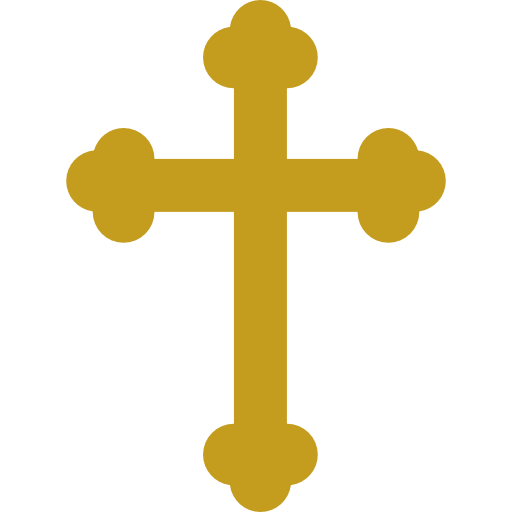
\includegraphics[scale=0.2]{./assets/cross.png} Santa Margarida de Cortona, rogai por nós!
}
% Place Page X of Y on the right-hand
% side of the footer
\fancyfoot[R]{\thepage}

\newpage

\tableofcontents

\centering
\vfill
Visite-nos no Telegram: \url{https://t.me/CotidieNovena}
\newpage

\newpage

%%%%%%%%%%%%%%%%%%%%%%%%%%%%%%%%%%%%% Orações %%%%%%%%%%%%%%%%%%%%%%%%%%%%%%%%%%%%%%%%%%%

\begin{justify}

 \begin{center}
  \section{História}\label{sec:História} % (fold)
 \end{center}

Santa Margarida de Cortona nasceu por volta do ano 1247 em uma pequena cidade Italiana chamada Laviano. Aos sete anos, Margarida sofre a morte de sua mãe.

Pouco tempo depois, o pai da Margarida se casou novamnte. Margarida não se dava bem com a nova madrasta, e essa, por sua vez, não gostava de Margarida.

Nos anos de sua adolescência, Margarida cresceu sendo muito teimosa. Ela ganhou a reputação de ser imprudente. Quando ela completou 17 anos, ela conheceu um homem nobre e decidiu fugir com ele.

O nobre não se casou com Margarida, mas a instalou em seu castelo como sua amante. Ela viveu com esse nobre por dez anos. Os dois tiveram um filho.

Um dia, o nobre não voltou de uma viagem no horário em que deveria voltar. Quando seu cão voltou para casa sem ele, Margarida ficou muito preocupada. O cão a levou até a floresta, onde ela descobriu o corpo morto de seu amante. Ela viu que ele havia sido assassinado.

O assassinato de seu amante afetou muito Margarida. Ela se arrependeu de seu estilo de vida e decidiu deixar a casa do nobre. Margarida levou seu filho com ela e tentou voltar para a casa do pai. No entanto, a madrasta de Margarida não a admitiu em sua casa.

Margarida e seu filho foram então para os frades franciscanos em Cortona. Lá, ela viveu uma vida de penitência. Ela jejuava com pão e vegetais e se dedicava à oração. Seu filho acabou se tornando um frade, e Margarida entrou para a Ordem Terceira de São Francisco. Ela logo começou a progredir em sua vida de oração.

Margarida desenvolveu uma devoção à Eucaristia e à Paixão de Jesus, e essas devoções a ajudaram a crescer em caridade. Ela imitou São Francisco de Assis, pedindo comida e servindo os pobres. Ela também fundou um hospital para os pobres. Ela também criou um grupo de irmãs da Terceira Ordem para servir como enfermeiras nesse hospital. 

Mais tarde, ela estabeleceu uma ordem de pessoas para servir aos necessitados e apoiar o hospital. Os membros dessa ordem eram devotos de Nossa Senhora da Misericórdia. Além disso, Margarida trabalhou para promover a reforma necessária na Igreja, desafiando seu bispo, que levava uma vida muito mundana. Margarida morreu em 1297. Após quatrocentos anos, seu corpo foi considerado incorrupto. Ela foi canonizada em 1728 pelo Papa Bento XIII.

\end{justify}

\vfill

\begin{center}
 \href{https://www.praymorenovenas.com/st-margaret-of-cortona-novena}{Fonte: Pray More Novenas}
\end{center}

%%%%%%%%%%%%%%%%%%%%%%%%%%%%%%%%%%%%% Orações %%%%%%%%%%%%%%%%%%%%%%%%%%%%%%%%%%%%%%%%%%%

\newpage
\begin{center}
 \section{Orações}\label{sec:Orações} % (fold)
\textit{Em nome do Pai, e do Filho, e do Espírito Santo. Amém.}
\end{center}

\subsection{Oração Incial}\label{sec:Oração_Inicial} % (fold)

Ó Gloriosa Santa Margarida de Corona, vós abraçastes a vida de penitência e pobreze depois de vos arrependerdes de vossos pecados.

Jesus tocou vosso coração, e depois de impor a si mesma uma vida de jejm rigorosa, Jesus falou e conversou convosco, revelando-vos Seu coração misericordioso que se alegra sempre que um pecador volta para Ele.

Por muitas penitências e jejuns, vós vos libertastes de todas as tentações, incluindo as da carne das quais fostes vítima por muitos anos.

Ouça aos nossos pedidos nesta novena \textbf{\textit{(mencione suas intenções aqui).}}

Amém.

\subsection{Oração Final}\label{sec:Oração_Final} % (fold)

\begin{center}
\textbf{Pai Nosso, Ave Maria, Glória ao Pai.}

Santa Margarida de Cortona, rogai por nós!
\end{center}

\subsection*{Créditos:}
\href{https://catholicnovenaapp.com/novenas/st-margaret-of-cortona-novena/#day-1-prayer}{Catholic Novena App}



\end{document}
